\chapter{Data}
\section{Image data for lossy compression}
Our end goal is for our method to be able to take an original image and compress it using lossy compression. In order to facilitate our method to have free reign in choosing which parts of the image data are discarded, we will not use images that have been compromised. This limits the types of images that we are willing to use, since images encoded in formats like JPEG, have been compromised. When going trough all papers listed in \cite{benchmark}, we found that most used the Kodak data set, containing 24 512x768 PNG images \cite{Kodak}. There where some other data sets used, most of which contained JPEG images. 24 images is not a huge amount when comparing with the amount of data used in some of the cutting edge deep learning image processing papers, one example being Google's FaceNet, where they had 260.000.000 images in the training set\cite{FaceNet}. 

Luckily due to an interest in photography, we have a private data set of about 10.000 3xxxX4xxx NEF images. These images are a lot larger than the the images in the Kodak data set, and would thus be more demanding of our computational resources. In order to lessen the computational load and be better able to compare ourselves with the literature, we will downsize our images to fit the Kodak image format of 512x768. By using combinations of cutting and downsizing the images, we can get the added benefit of also increasing our data set.

To make the images 512x768, we start by trimming the edges, in order for the x axes to be divisible by 768 and the y axes to be divisible by 512. Then the image gets cut into peaces as can be seen in the following figure:
\begin{figure}[H]
    \centering
    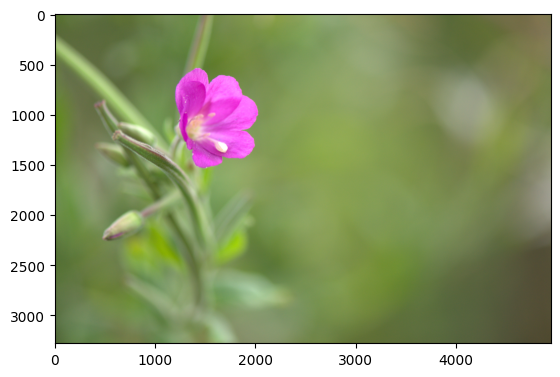
\includegraphics[width=0.45\linewidth,origin=c]{Report/Pictures/data/Original_img.png}
    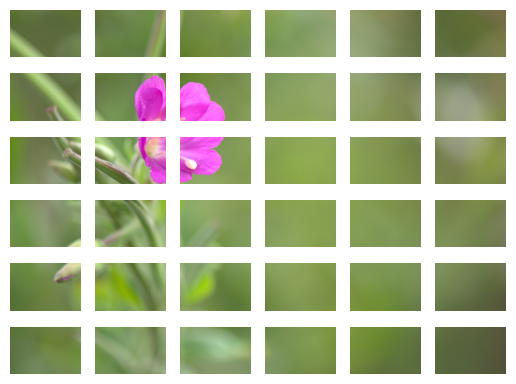
\includegraphics[width=0.45\linewidth,origin=c]{Report/Pictures/data/Split_img.png}
    \caption{Cutting of the original image}
\end{figure}

Afterwards the trimmed image gets downsized and cut again, until it is no longer possible. This can be seen in the following figure:

\begin{figure}[H]
    \centering
    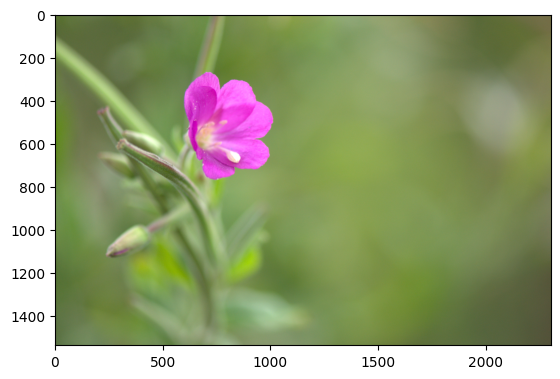
\includegraphics[width=0.45\linewidth,origin=c]{Report/Pictures/data/reduced_img.png}
    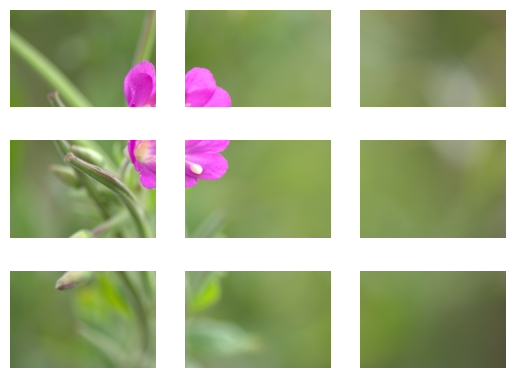
\includegraphics[width=0.45\linewidth,origin=c]{Report/Pictures/data/Reduced_and_split.png}

    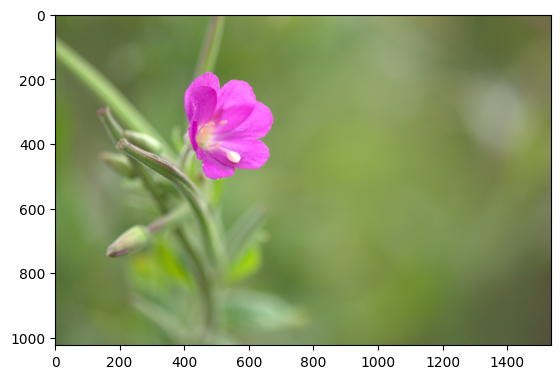
\includegraphics[width=0.45\linewidth,origin=c]{Report/Pictures/data/reduced_2x2.png}
    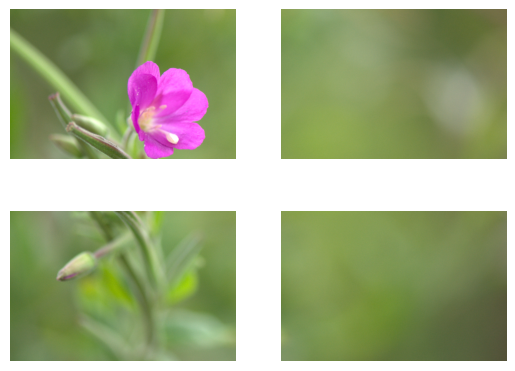
\includegraphics[width=0.45\linewidth,origin=c]{Report/Pictures/data/2x2.png}

    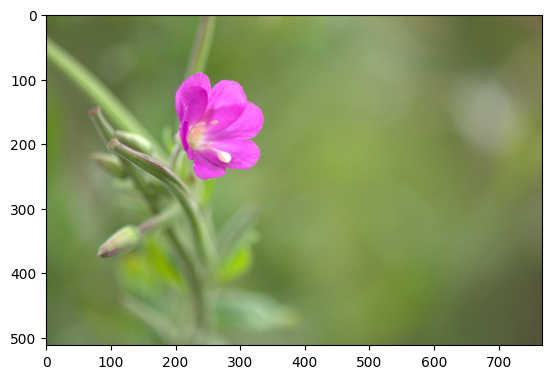
\includegraphics[width=0.90\linewidth,origin=c]{Report/Pictures/data/reduced_1x1.png}

    \caption{Further cutting of the original image}
\end{figure}

After this procedure, there are 50 images for each original image, leading to there being about 500.000 images in total. Many further transformations of the images are possible, these include rotations of the color channels, flipping and rotating the images, sharing etc. We only apply flipping and rotation of the images, these can be seen below:

\begin{figure}[H]
    \centering
    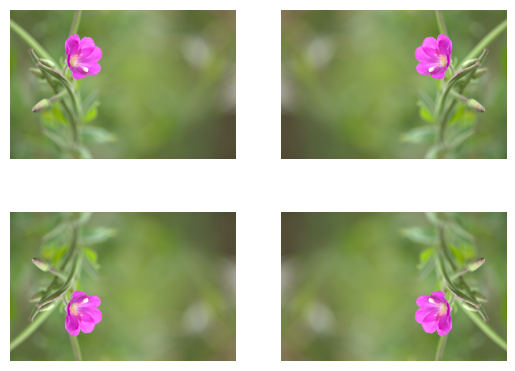
\includegraphics[width=0.90\linewidth,origin=c]{Report/Pictures/data/Flips.png}
    \caption{Flips of image}
\end{figure}

This further increases the set of images by a factor of 4, leading to a training set of about 2.000.000 images. 2.000.000 images is only 1\% of the amount used in \cite{FaceNet}, however, our computational resources and patience would likely be insufficient to handle many more images. 

We are also using the Kodak data set, in order to compare our results with the literature.




\subsection{Image data for neural loss function}

In order to make a neural network that can distinguish between good and bad reconstructions of images, we need a data set containing good and bad reconstructions of images along with the original image. We do not have access to any such data set and it is infeasible to create one due to time and monetary constraints. 
Instead, we build different augmentation functions, that augment the images in various ways to various degrees. Each of these functions gets scored by us, in terms of how acceptable the transformation is. Thus for every setting of every function we grade, we get one "reconstruction" of the original image of that grade. The transformations are further discussed in section SECTIONSECTIONSECTIONSECTION.
